\documentclass[twoside,12pt]{article}
\usepackage{url}
\usepackage{amsmath,amsfonts,amsthm,fullpage,amssymb}
\usepackage{algorithm}
\usepackage{algorithmic}
\usepackage{graphicx}
\usepackage{float}
\usepackage{multirow}
\usepackage{subcaption}
\usepackage[colorlinks=true, hidelinks]{hyperref}
\usepackage{enumitem}
\usepackage{tcolorbox}
\hypersetup{
    colorlinks=true,
    linkcolor=blue,
    citecolor=blue,
}
\usepackage{listings}
\usepackage{xcolor}

\definecolor{codegreen}{rgb}{0,0.6,0}
\definecolor{codegray}{rgb}{0.5,0.5,0.5}
\definecolor{codepurple}{rgb}{0.58,0,0.82}
\definecolor{backcolour}{rgb}{0.95,0.95,0.92}

% \makeatletter
% \renewcommand{\@makefnmark}{%
%   \hbox{%
%     \@textsuperscript{%
%       \normalfont\color{blue}(\@thefnmark)%
%     }%
%   }%
% }
% \makeatother

\lstdefinestyle{mystyle}{
    backgroundcolor=\color{backcolour},   
    commentstyle=\color{codegreen},
    keywordstyle=\color{magenta},
    numberstyle=\tiny\color{codegray},
    stringstyle=\color{codepurple},
    basicstyle=\ttfamily\footnotesize,
    breakatwhitespace=false,         
    breaklines=true,                 
    captionpos=b,                    
    keepspaces=true,                 
    numbers=left,                    
    numbersep=5pt,                  
    showspaces=false,                
    showstringspaces=false,
    showtabs=false,                  
    tabsize=2
} 

\lstset{style=mystyle}

\usepackage[backend=biber,style=alphabetic,sorting=ynt]{biblatex}
\addbibresource{references.bib}

\begin{document}


\title{ISYE 6740, Fall 2025, Homework 3\\{\small 100 points + 10 bonus points}\\}
\author{Will Pickard}
%\author{Yao Xie}
\date{}
\maketitle

\textbf{Provided Data:} \\
Questions marked with GS must be submitted to Gradescope. You must still include all your results and explanations in this PDF, and include your code in your canvas submission to receive credit. Failure to pass all gradescope tests will result in a 50\% penalty to the points for that question.

\textbf{This assignment does not have any gradescope requirements}

\begin{itemize}
    \item Q2: Density Estimation: Psychological experiments [n90pol.csv]
    \item Q3: Implementing EM for MNIST Dataset [data.dat, data.mat, label.mat, label.dat]
\end{itemize}

\subsection*{1. Conceptual questions. [20 points]}


\begin{enumerate}[label*=\arabic*.]
\item (5 points) Please compare the pros and cons of KDE over histogram, and give at least one advantage and disadvantage to each.
\subsubsection{KDE Pros and Cons}
\textbf Advantages
\begin{itemize}
    \item Smooth estimate output can reveal patterns in the data more granularly, such as multiple peaks in the data where a histogram might not catch that.
    \item Does not require an assumption about the underlying data distribution.
\end{itemize}
\textbf Disadvantages
\begin{itemize}
    \item Kernel summation can give the impression that data exists at false points.
    \item More computationally intense than a histogram, especially with large number of samples.
\end{itemize}

\subsubsection{Histogram Pros and Cons}
\textbf Advantages
\begin{itemize}
    \item Histograms are simple to calculate and simple to interpret for stakeholders that may not be very technical.
    \item Does not require an assumption about the underlying data distribution.
\end{itemize}
\textbf Disadvantages
\begin{itemize}
    \item The choices in binning parameters can have a large impact on distribution representation. This can cause noise in the representation
    \item Not sample efficient for high-dimensional data. If the number of bins $(\frac{1}{\Delta})^n$ is larger than sample size, many bins are empty.
\end{itemize}

\item (5 points) Explain why the maximum likelihood estimation (MLE) cannot be applied directly to estimate the parameters of a GMM. Additionally, what is the standard approach used to fit a GMM effectively?
 
The GMM function relies on the unobserved latent variables $z_i$ which basically indicates the Gaussian kernel to which the data point belongs. MLE would be feasible if the latent variables were known, since they are not, MLE would have to integrate over all possible values of $Z$. The log-likelihood function for GMM is:
$$l(\theta;D) = \log \prod_{i=1}^m\left(\sum_{k=1}^K p\left(x^i, z^i=k \mid \theta\right)\right)$$ 

The problem arises from the summation of $k$ inside the logarithm. Unlike with a single Gaussian, setting the derivative to zero (as in MLE) will not yield a closed form solution (\cite{bishop2007} p.435).

Instead, the standard approach to fitting GMM is the EM (Expectation-Maximization) algorithm. $K$ gaussians are instantiated. Then, during the Expectation step, we calculate the probability of each data point belonging to one of the $K$ gaussians. This is repeated for every gaussian. Then, the Maximization step performs a weighted MLE for each cluster to recalculate the gaussian parameters $(\pi_k, \mu_k, \Sigma_k)$. Then, the steps are continuously repeated until the algorithm converges.

The steps here can be heavily compared to K-Means clustering. The key difference is that fitting a GMM produces soft-assignments of the data points. Unlike K-means, which produces one cluster assignment for each point, GMM produces that likelihood that a point belongs to each gaussian (a soft-assignment). Therefore, a point can belong 40\% to one cluster and 60\% to another.

\item (5 points) For the EM algorithm for GMM, please show how to use the Bayes rule to derive $\tau_k^i$ in a closed-form expression.

$\tau_k^i$ is called the "responsibility," which represents the probability that the latent variable $z_i$ is in cluster k given the data point $x_i$ and model parameters $\Theta$. EM uses this derivation during the Expectation step to solve the issue of incomplete data. In order to fit the gaussians with the correct parameters using maximum likelihood, we would need the complete data in the joint distribution $p(X,Z|\Theta)$. Since we only have data on $X$, we supplant knowledge of Z with its expected value under the posteriior distribution of the latent variable (\cite{bishop2007} p. 440). With this posterior distribution supplanting direct information on the latent variables, the maximization step can use maximum likelihood to fit the gaussian parameters that fit the $p(X, Z_{current} | \Theta)$ distribution. By iterating this process, EM arrives at a local maximum that soft-assigns the data to K gaussian distributions. 
Bayes rule is:
\begin{align*}
P(z|x) &= \frac{P(x|z)P(z)}{P(x)} \\
\intertext{Which corresponds to:} \\
\text{Posterior} &= \frac{\text{Likelihood} \times \text{Prior}}{\text{Normalization constant}} = \frac{P(x,z)}{\sum_{z'}P(x,z')} \\
\text{where } P(z) &= \pi_z ; \quad P(x|z)=\mathcal{N}(x|\mu_z,\Sigma_z); \quad p(x) = \sum_{z=1}^K p(x|z)p(z)\\
\intertext{Plugging in these distribution definitions:} \\
P(z|x) &= \frac{\pi_z \mathcal{N}(x|\mu_z,\Sigma_z)}{\Sigma_{z'}\pi_{z'}\mathcal{N}(x|\mu_{z'},\Sigma_{z'})}
\end{align*}

Given that general definition, we can apply it to all of our data points in X to get the full posterior distribution of the latent variables Z.

\begin{align*}
q(z^1...z^m) &= \prod_{i=1}^m p(z^i | x^i, \Theta^t)
\end{align*}

Basically, this allows us to solve the posterior per data point $x^i$ to find the corresponding latent variable for that point $z^i$ across all $K$ potential values of $z^i$. This is expressed by:

\begin{align*}
\tau_k^i &= p(z^i = k|x^i,\Theta^t) = \frac{p(x^i|z^i = k)p(z^i=k)}{\sum_{k'=1...K}p(z^i=k', x^i)} = \frac{\pi_k \mathcal{N}(x^i|\mu_k,\Sigma_k)}{\sum_{k'=1...K}\pi_{k'} \mathcal{N}(x^i|\mu_{k'},\Sigma_{k'})}
\end{align*}

Perhaps the name of the $\tau_{k^i}$ variable describes this expression best - the responsibility. $\tau_{k^i}$ represents the probability that the data point $x^i$ belongs to the $k^{th}$ gaussian, basically the probability that the gaussian is "responsible" for that data point.


\item (5 points) Based on the outline given in the lecture, show that the maximum likelihood estimate (MLE) for Gaussian random variable using $n$-dimensional observations $x^1, \ldots, x^m$, that are {\it i.i.d.} (independent and identically distributed) following the distribution $\mathcal N(\mu, \Sigma)$, and the mean and variance parameters are given by 
\[
\hat \mu = \frac 1 m \sum_{i=1}^m x^i, \quad \hat \Sigma = \frac 1 m \sum_{i=1}^m (x^i - \hat \mu)(x^i - \hat \mu)^T,
\]
respectively. Please show the work for your derivations in full detail. Discuss what is the rank of $\hat \Sigma$ when $m<n$? In the extreme case, when $m=1$ (i.e., only one sample), what is the rank of $\hat \Sigma$? This question shows that, when the data is high-dimensional, the sample size needs to be sufficiently large relative to the dimension (otherwise we need special treatment to handle low-rank covariance matrix.)

Performing with the n-Dimensional Gaussian:
\begin{align*}
    \mathcal{N}(X|\mu,\Sigma) &= \frac{1}{\sqrt{|\Sigma|}(2\pi)^{\frac{n}{2}}}e^{-\frac{1}{2}(X-\mu)^T\Sigma^{-1}(X-\mu)}\\
    \intertext{The likelihood equation is given by the product of the PDF for each i.i.d data point in vectors $D = {x^1,x^2...x^m}$:}\\
    L (\mathcal{N}(X|\mu,\Sigma)) &= \prod_{i=1}^m \frac{1}{\sqrt{|\Sigma|}(2\pi)^{\frac{n}{2}}}e^{-\frac{1}{2}(X-\mu)^T\Sigma^{-1}(X-\mu)}
\end{align*}
Taking the log likelihood allows us to convert the product into a summation due to the above log property. Since log is monotonic, it preserves the order of magnitudes of the function, which allows the $\mu$ and  $\Sigma$ that produce a maximized log likelihood are also the values that produce the maximized likelihood.
\begin{align*}
    l (\mathcal{N}(X|\mu,\Sigma)) &= \log(L) = \log\prod_{i=1}^m \frac{1}{\sqrt{|\Sigma|}(2\pi)^{\frac{n}{2}}}e^{-\frac{1}{2}(X-\mu)^T\Sigma^{-1}(X-\mu)}\\
    \intertext{Applying log properties:}\\
    &= \sum_{i=1}^m[ \log{1} -\log{|\Sigma|^{\frac{1}{2}}} - \log{2\pi^{\frac{n}{2}}} + \log{e^{-\frac{1}{2}(x^i-\mu)^T\Sigma^{-1}(x^i-\mu)}}]\\
    &=  0 - \sum_{i=1}^m\frac{1}{2}\log{|\Sigma|} - \sum_{i=1}^m\frac{n}{2}\log{2\pi} - \sum_{i=1}^m \frac{1}{2}(x^i-\mu)^T\Sigma^{-1}(x^i-\mu)\\
    \intertext{For terms without $i$, the summations are equivalent to multiplying by $m$:}
    l(\mu,\Sigma;D)&=  -\frac{m}{2}\log{|\Sigma|} - \frac{mn}{2}\log{2\pi} - \frac{1}{2}\sum_{i=1}^m (x^i-\mu)^T\Sigma^{-1}(x^i-\mu)\\
\end{align*}
Now we can take the partial derivatives with respect to $\mu$ and $\Sigma$ and set them equal to zero. This gives the values at which the likelihood is maximized. First, some properties we will need.
\begin{align}
    \text{Matrix derivative property (\cite{Petersen2008} eq 82)}: \frac{\partial}{\partial s}(x - s)^T W(x - s) = -2W(x-s) \\
    \text{Trace property (\cite{Petersen2008} eq 16)}: Tr(ABC) = Tr(BCA) = Tr(CAB) \\
    \text{Trace derivative property (\cite{Petersen2008} eq 100)}: \frac{\partial}{\partial X}Tr(XA) = A^T \\
    \text{Determinate log derivative (\cite{Petersen2008} eq. 57):} \frac{\partial (ln(|X|))}{\partial X} = (X^{-1})^T = (X^T)^{-1}
\end{align}
Finding $\hat{\mu}$:
\begin{align*}
    \frac{\partial l}{\partial \mu} = 0 &= -\frac{1}{2}\sum_{i=1}^m[-2\Sigma^{-1}(x^i-\mu)] \\
    0 (\Sigma) &= (\Sigma)\Sigma^{-1}\sum_{i=1}^m(x^i-\mu) \\
    0 &= \sum_{i=1}^m x^i - m\mu \\
    \hat{\mu} &= \frac{1}{m}\sum_{i=1}^m x^i\\
\end{align*}

Finding $\hat{\Sigma}$ requires using the trace derivative property and the determinate log derivative. According to a Stackexchange post (\cite{se351550}), the trace is used because $x^TAx$ will be scalar, meaning we can arrive at the same value from the trace. We also use the trace properties to reconfigure the terms within the trace so we can use the derivative property.

\begin{align*}
    \frac{\partial l}{\partial \Sigma} = 0 &= -\frac{\partial}{\partial \Sigma}\frac{m}{2}\log{|\Sigma|} -\frac{1}{2}\sum_{i=1}^m\frac{\partial}{\partial \Sigma}(Tr((x^i-\mu)^T\Sigma^{-1}(x^i-\mu))) \\
    0 &= -\frac{\partial}{\partial \Sigma}\frac{m}{2}(-1)(-1)\log{|\Sigma|} -\frac{1}{2}\sum_{i=1}^m\frac{\partial}{\partial \Sigma}(Tr((x^i-\mu)^T\Sigma^{-1}(x^i-\mu))) \\
    0 &= -\frac{\partial}{\partial \Sigma}\frac{m}{2}(-1)\log{|\Sigma^{-1}|} -\frac{1}{2}\sum_{i=1}^m\frac{\partial}{\partial \Sigma}(Tr((x^i-\mu)^T\Sigma^{-1}(x^i-\mu))) \\
    0 &= \frac{m}{2}(\Sigma^T) -\frac{1}{2}\sum_{i=1}^m\frac{\partial}{\partial \Sigma}(Tr((x^i-\mu)(x^i-\mu)^T\Sigma^{-1})) \\
    0 &= \frac{m}{2}(\Sigma^T) -\frac{1}{2}\sum_{i=1}^m(x^i-\mu)(x^i-\mu)^T \\
    0 &= \frac{m}{2}(\Sigma) -\frac{1}{2}\sum_{i=1}^m(x^i-\mu)(x^i-\mu)^T; \quad \text{since $\Sigma = \Sigma^T$} \\
    -\frac{m}{2}(\Sigma) &= -\frac{1}{2}\sum_{i=1}^m(x^i-\mu)(x^i-\mu)^T\\
    \Sigma &= \frac{1}{m}\sum_{i=1}^m(x^i-\mu)(x^i-\mu)^T\\
    \intertext{Replace $\mu$ with $\hat{\mu}$ because both values must be maximized for optimal solution.}
    \hat{\Sigma} &= \frac{1}{m}\sum_{i=1}^m(x^i-\hat{\mu})(x^i-\hat{\mu})^T\\
\end{align*}

The rank of a matrix is the number of linearly independent rows or columns in the data. The $x^i$ vector is $nx1$ and therefore rank-1. The outer product matrix $(x^i-\hat{\mu})(x^i-\hat{\mu})^T$ will also have rank-1, since it's comprised of multiplicatiosn of the same rank-1 vector. Summing $m$ rank-1 outer product matrices should have a maximum rank of $m$ (\cite{se180366}). However, the mean value incorporated in $\hat{\mu} = \frac{1}{m}\sum_{i=1}^m x^i$ changes the maximum rank of $\hat{\Sigma} \le m-1$.

\begin{align*}
    \text{Let } \quad z^i &= (x^i-\hat{\mu}) \\
     &= \sum_{i=1}^m(x^i) - m\hat{\mu} \\
     &= \sum_{i=1}^m(x^i) - m\hat{\mu} \\
     \text{Knowing} \quad \hat{\mu} &= \frac{1}{m}\sum_{i=1}^m x^i\\
     \sum_{i=1}^m z^i &= m\hat\mu - m\hat{\mu} = 0\\
     z^m &= -\sum_{i=1}^{m-1} z^i\\
\end{align*}

So, the summation is not completely independent - since the sum must equal zero, any vector can be constructed as a linear combination of the other vectors. This means the rank of the summation must be $\le m-1$. Since $\hat\Sigma$ is comprised of $ZZ^T$, its rank cannot be greater than the subspace of $Z$, so Rank$(\hat\Sigma) \le m-1$.

When $m<n$, the rank of $\hat\Sigma \le m-1 < n$. So the rank of the $nxn$ matrix $\hat\Sigma$ is less than its dimension, which means the matrix is singular and therefore non-invertible. This is a major problem, since the n-dimensional Gaussian distribution requires $\Sigma^{-1}$.

In the extreme case $m=1$, the mean $\hat\mu = x^1$. By the definitions of $\hat\mu = x^1$ and $\hat\Sigma=(0)(0)^T$. Logically, with a single data point, there is no "distribution" to really consider.

\end{enumerate}

\subsection*{2. Density estimation: Psychological experiments. [25 points]}


In {\it Kanai, R., Feilden, T., Firth, C. and Rees, G., 2011. Political orientations are correlated with brain structure in young adults. Current biology, 21(8), pp.677-680.}, data are collected to  study whether or not the two brain regions are likely to be independent of each other and considering different types of political view \textbf{For this question; you can use third party histogram and KDE packages; no need to write your own.} The data set \textsf{n90pol.csv} contains information on 90 university students who participated in a psychological experiment designed to look for relationships between the size of different regions of the brain and political views. The variables \textsf{amygdala} and \textsf{acc} indicate the volume of two particular brain regions known to be involved in emotions and decision-making, the amygdala and the anterior cingulate cortex; more exactly, these are residuals from the predicted volume, after adjusting for height, sex, and similar body-type variables. The variable \textsf{orientation} gives the students' locations on a five-point scale from 1 (very conservative) to 5 (very liberal).  Note that in the dataset, we only have observations for orientation from 2 to 5. 

Recall in this case, the kernel density estimator (KDE) for a density is given by
 \[
 p(x) = \frac 1 m \sum_{i=1}^m \frac 1 h
 K\left(
 \frac{x^i - x}{h}
 \right),
 \]
where $x^i$ are two-dimensional vectors, $h >0$ is the kernel bandwidth, based on the criterion we discussed in lecture. 
For one-dimensional KDE,  use a one-dimensional Gaussian kernel
\[
K(x) = \frac{1}{\sqrt{2\pi}} e^{-x^2/2}.
\]
For two-dimensional KDE, use a two-dimensional Gaussian kernel: for \[x = \begin{bmatrix}x_1\\x_2\end{bmatrix}\in \mathbb R^2,\] where $x_1$ and $x_2$ are the two dimensions respectively \[K(x) = \frac{1}{2\pi} e^{-\frac{(x_1)^2 + (x_2)^2}{2}}.\] 
  
 \begin{enumerate}[label*=\arabic*.]
 
 
 \item (5 points) Form the 1-dimensional histogram and KDE to estimate the distributions of \textsf{amygdala} and \textsf{acc}, respectively. For this question, you can ignore the variable \textsf{orientation}. Decide on a suitable number of bins so you can see the shape of the distribution clearly. Set an appropriate kernel bandwidth $h >0$. 
 
 The histogram and KDEs are shown below. I used Silverman's rule of thumb (\cite{enwiki:1305066115})to calculate the optimal bandwidth, then compared the output with the half, 1.5, and twice optimal bandwidth permutations. I used the Freedman-Diaconis rule (\cite{se862}) to calculate the optimal number of bins for the histograms, then experimented with the same permutations of the bins. In all cases, the calculated optimal numbers seemed most serviceable, so I've kept this pattern throughout this entire question. For the histograms, the calculated optimal bins graph is second from the top. For KDE, the calculated optimal BW is third from the top. 

    \begin{figure}[H]
        \centering
        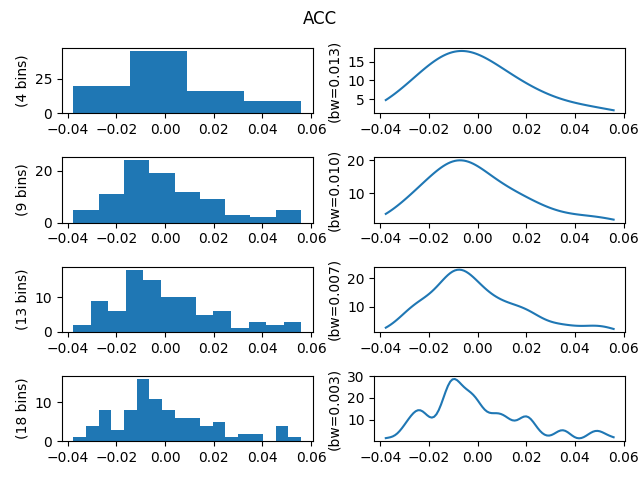
\includegraphics[width=\textwidth]{images/1D_ACC.png}
    \end{figure}
    \begin{figure}[H]
        \centering
        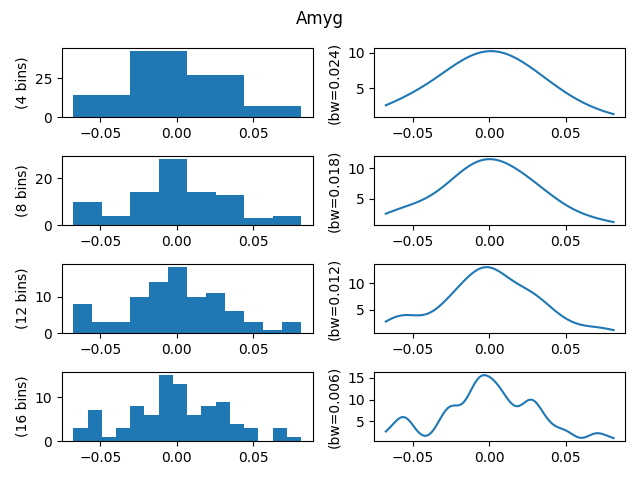
\includegraphics[width=\textwidth]{images/1D_Amyg.png}
    \end{figure}

 \item (5 points) Form 2-dimensional histogram for the pairs of variables (\textsf{amygdala}, \textsf{acc}). Decide on a suitable number of bins so you can see the shape of the distribution clearly. 

 The 2D histogram is included in the next question figure.
 
 \item (5 points) Use kernel-density-estimation (KDE) to estimate the 2-dimensional density function of (\textsf{amygdala}, \textsf{acc}) (this means for this question, you can ignore the variable \textsf{orientation}). Set an appropriate kernel bandwidth $h>0$. Keep in mind that your choice of bandwidth can heavily affect your distributions, and you should be experimenting to ensure you are capturing the true distribution.
 

Please show the two-dimensional KDE (e.g., two-dimensional heat-map, two-dimensional contour plot, etc.)

Please explain what you have observed: is the distribution unimodal or bi-modal? Are there any outliers? 

Are the two variables (\textsf{amygdala}, \textsf{acc}) likely to be independent or not? Please support your argument with reasonable investigations.

The 2D histogram and KDE are shown below. For the histogram, I matched the bins along each axis with the optimal bin numbers determined in question $2.1$. For the KDE, I used the built-in Silverman's rule of thumb \lstinline{bw_method} provided in sci-kit learn's KernelDensity estimator.

    Judging from the 1D KDE plots, the built-in BW calculation seemed on-par. I also included a figure using $0.75 \times BW$ to see a less smoothed plot, but I think the automatically calculated BW is best. Again, this pattern held for the later questions, so this strategy was used for all the joint distributions in ensuing questions.

    \begin{figure}[H]
        \centering
        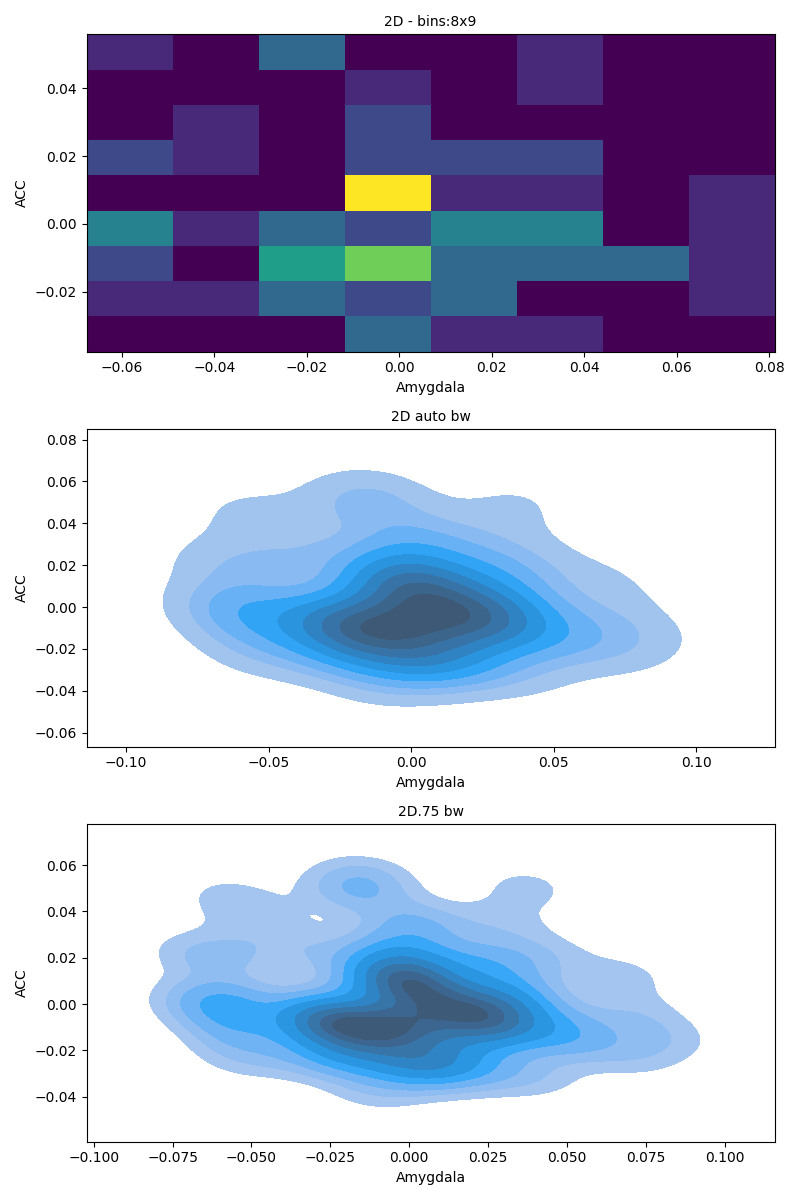
\includegraphics[width=\textwidth, height=\textwidth]{images/2D_2D.png}
    \end{figure}

    The graphs show that the joint distribution is unimodal with some slight outliers. The outliers are shown in the histogram as lighter colored bins away from the center and as darker pockets away from the very dark middle on the KDE plots (most visible on the .75BW plot). It's also unlikely that the variables are independent, since there seems to be a slight positive correlation in the two variables. This is seen in the dense middle, which is elliptical in the north east direction. This correlation means that there's a tendency for ACC to increase as Amygdala increases. 


 \item (5 points) We will consider the variable \textsf{orientation} and consider conditional distributions. Please plot the estimated conditional distribution of \textsf{amygdala} conditioning on political \textsf{orientation}: $p(\textsf{amygdala}|\textsf{orientation}=c)$, $c = 2, \ldots, 5$, using KDE. Set an appropriate kernel bandwidth $h >0$.  Do the same for the volume of the \textsf{acc}: plot $p(\textsf{acc}|\textsf{orientation}=c)$, $c = 2, \ldots, 5$ using KDE. (Note that the conditional distribution can be understood as fitting a distribution for the data with the same $\textsf{orientation}$. Thus you should plot 8 one-dimensional distribution functions in total for this question.) 
 
 I used the same bandwidth calculations and comparisons as prior, so the optimal bandwidth is the third from the top. I plotted the 1D ACC and Amygdala graphs side-by-side for comparison.

 \begin{figure}[H]
        \centering
        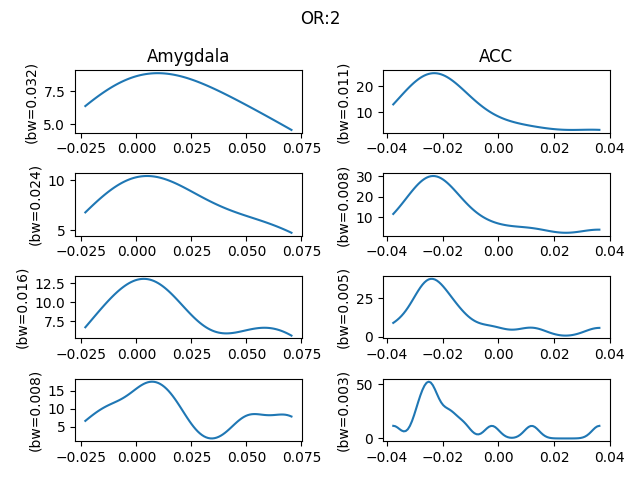
\includegraphics[width=\textwidth, height=\textwidth]{images/1D OR2 amyg+acc.png}
    \end{figure}
 \begin{figure}[H]
        \centering
        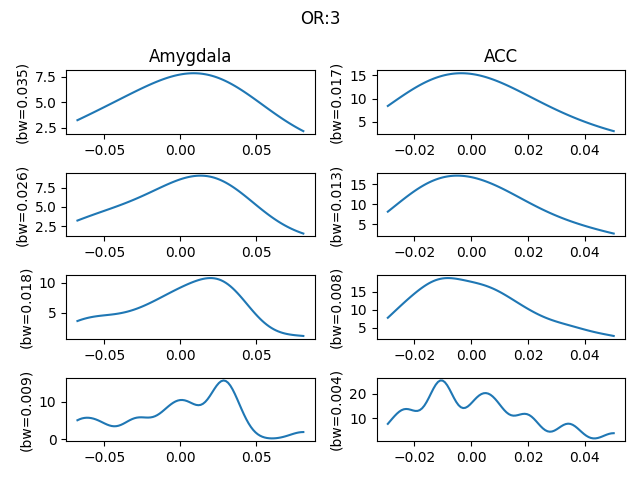
\includegraphics[width=\textwidth, height=\textwidth]{images/1D OR3 amyg+acc.png}
    \end{figure}
 \begin{figure}[H]
        \centering
        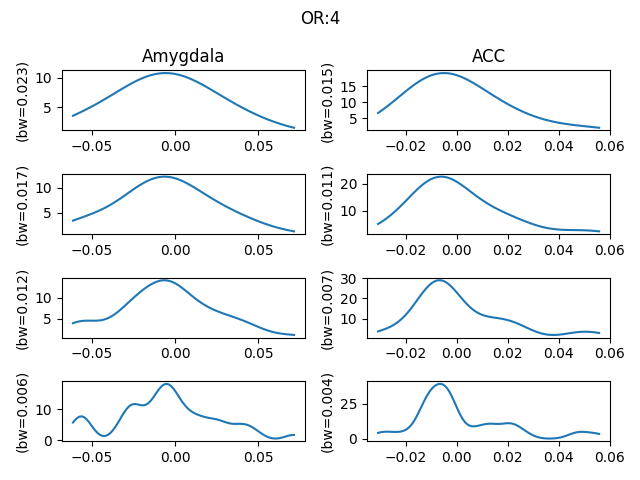
\includegraphics[width=\textwidth, height=\textwidth]{images/1D OR4 amyg+acc.png}
    \end{figure}
 \begin{figure}[H]
        \centering
        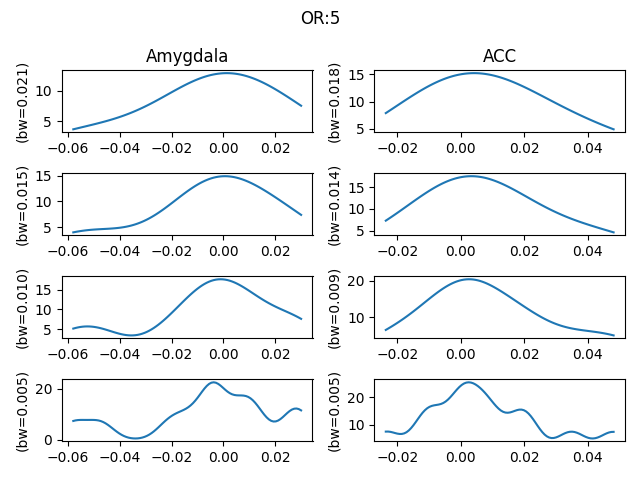
\includegraphics[width=\textwidth, height=\textwidth]{images/1D OR5 amyg+acc.png}
    \end{figure}

 
Now please explain based on the results, can you infer that the conditional distribution of  \textsf{amygdala} and \textsf{acc}, respectively, are different from $c = 2, \ldots, 5$? This is a type of scientific question one could infer from the data: Whether or not there is a difference between brain structure and political view.

There doesn't seem to be a clear correlation between the political view and the brain structures. Comparing the orientation graphs, there isn't a trend that seems consistent. The centering of the graphs tends to be around 0, and while there are fluctuations in that, they aren't consistent in direction as the political direction shifts.

Now please also fill out the {\it conditional sample mean} for the two variables: %
\begin{center}
\begin{tabular}{|c|c|c|c|c|}
\hline
& $c = 2$ & $c = 3$ & $c = 4$ & $c = 5$ \\\hline
\textsf{amygdala} & 0.019 &0.001 &-0.006 & -0.005\\\hline
\textsf{acc} & -0.015&0.002 & 0.008& 0.001\\\hline
\end{tabular}
\end{center}
Remark: As you can see this exercise, you can extract so much more information from density estimation than simple summary statistics (e.g., the sample mean) in terms of explorable data analysis.  
 
 \item (5  points) Again we will consider the variable \textsf{orientation}. We will estimate the conditional {\it joint} distribution of the volume of the \textsf{amygdala} and \textsf{acc}, conditioning on  a function of political \textsf{orientation}: $p(\textsf{amygdala}, \textsf{acc}|\textsf{orientation}=c)$, $c = 2, \ldots, 5$. You will use two-dimensional KDE to achieve the goal; et an appropriate kernel bandwidth $h >0$. Please show the two-dimensional KDE (e.g., two-dimensional heat-map, two-dimensional contour plot, etc.). 
 
 I generated the plot in the same fashion as with the non-conditioanl joint distributions.

  \begin{figure}[H]
        \centering
        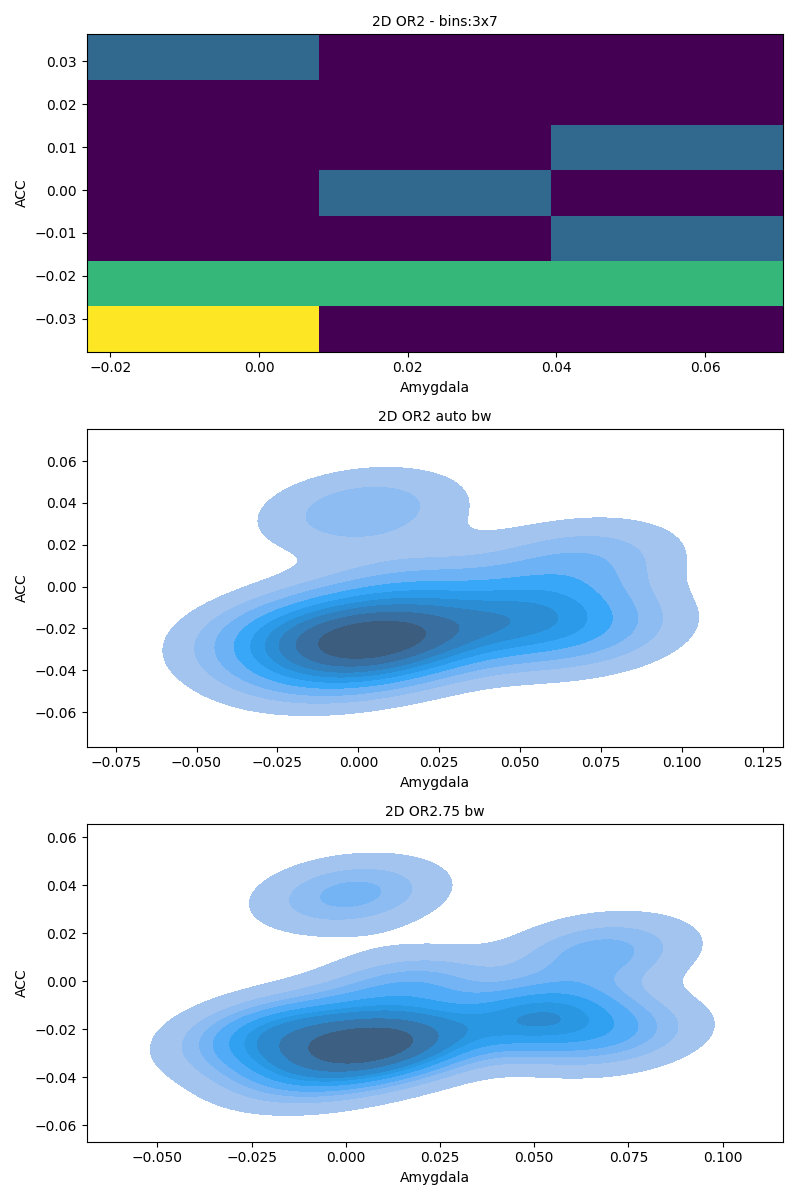
\includegraphics[width=\textwidth, height=\textwidth]{images/2D_2D OR2.png}
    \end{figure}
  \begin{figure}[H]
        \centering
        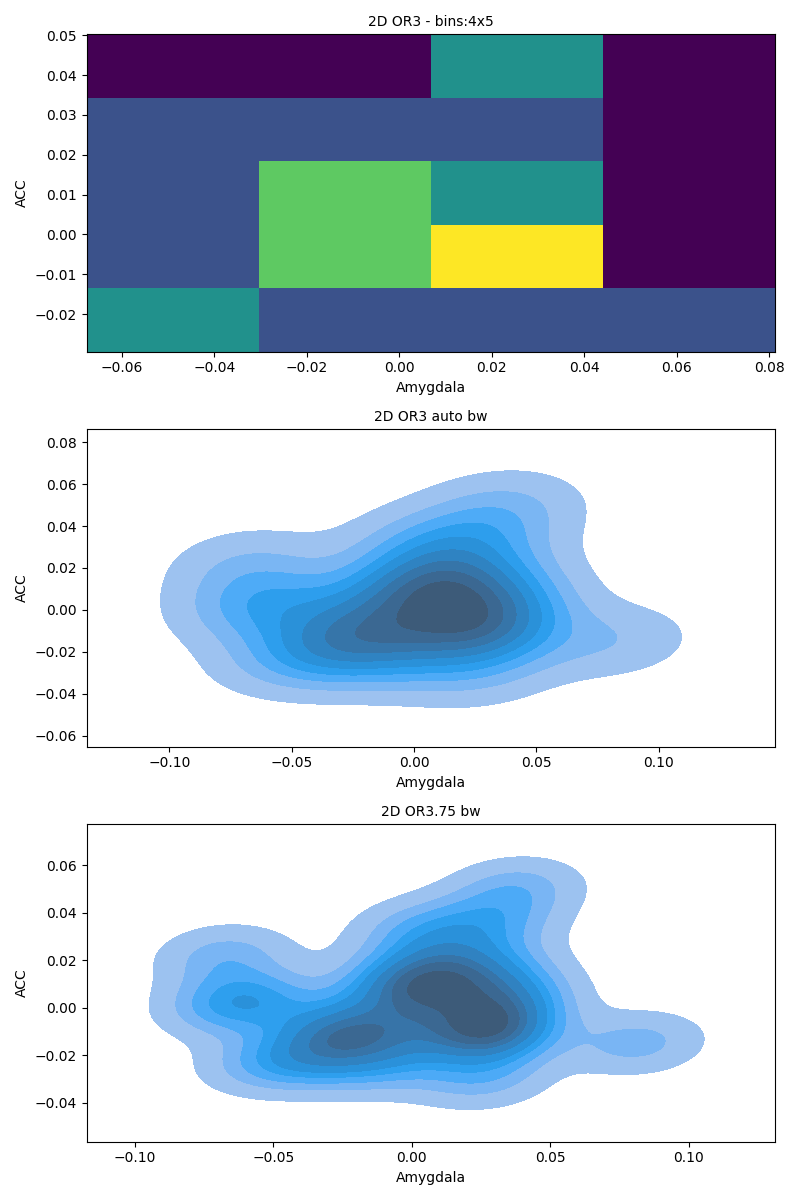
\includegraphics[width=\textwidth, height=\textwidth]{images/2D_2D OR3.png}
    \end{figure}
  \begin{figure}[H]
        \centering
        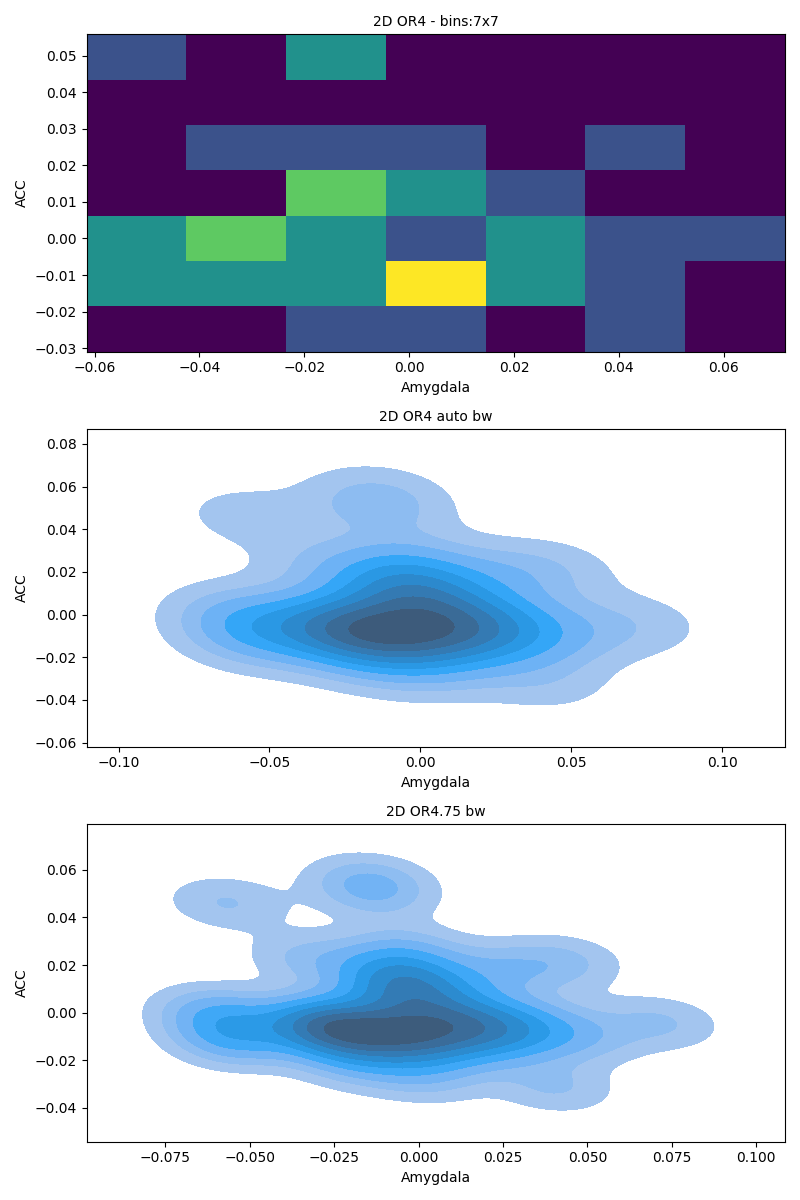
\includegraphics[width=\textwidth, height=\textwidth]{images/2D_2D OR4.png}
    \end{figure}
  \begin{figure}[H]
        \centering
        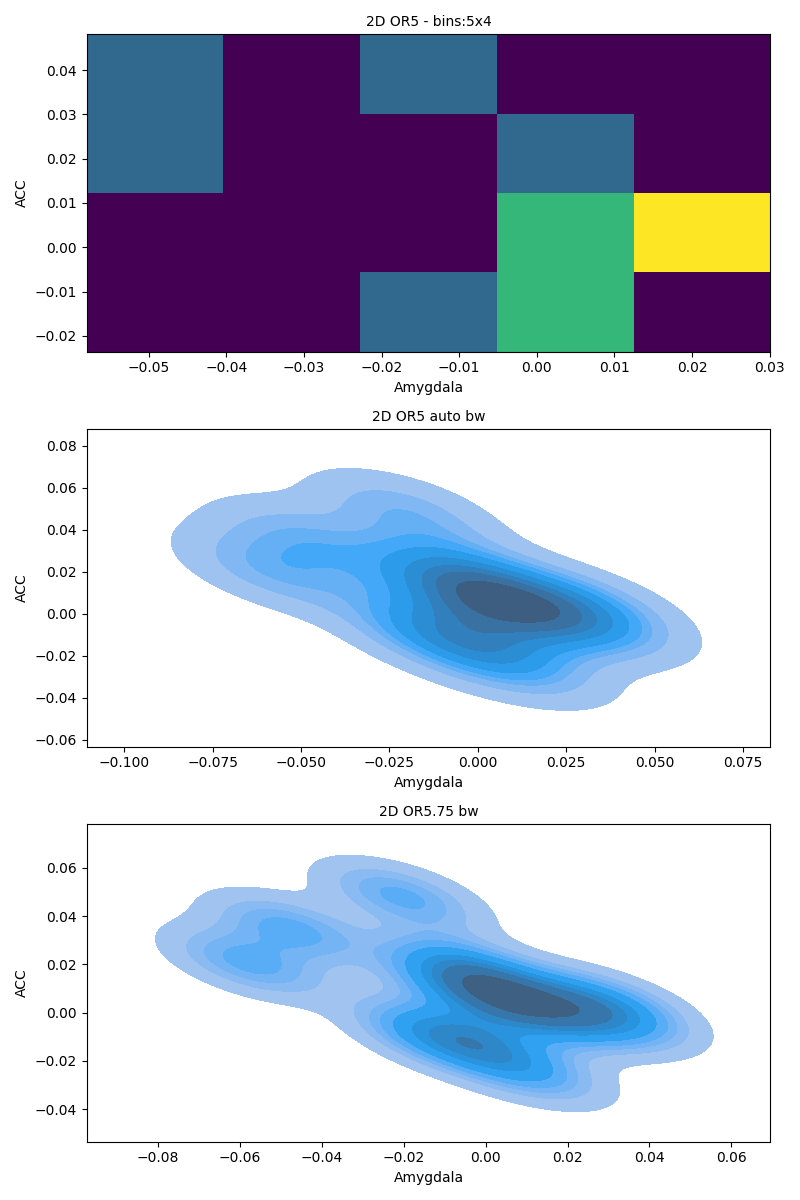
\includegraphics[width=\textwidth, height=\textwidth]{images/2D_2D OR5.png}
    \end{figure}
 
 Please explain based on the results, can you infer that the conditional distribution of two variables (\textsf{amygdala}, \textsf{acc}) are different from $c = 2, \ldots, 5$? This is a type of scientific question one could infer from the data: Whether or not there is a difference between brain structure and political view.
 
 The conditional joint distributions don't show clear political orientation by brain structure. There seems to be a slight positive correlation for orientation 2 and a slight negative correlation for orientation 5. However, this pattern is likely due to noise. The centering of the peak in the distributions doesn't seem to move in a clear pattern. It would be helpful to have orientation 1 in the dataset, but judging from this analysis, I don't think there's a clear way to determine political orientation from these brain structures.
  
 \end{enumerate}
 

\subsection*{3. Implementing EM for MNIST dataset. [40 points]}

Implement the EM algorithm for fitting a Gaussian mixture model for the MNIST handwritten digits dataset. For this question, we reduce the dataset to be only two cases, of digits ``2'' and ``6'' only. Thus, you will fit GMM with $C = 2$. Use the data file \textsf{data.mat} or \textsf{data.dat}. True label of the data are also provided in \textsf{label.mat} and \textsf{label.dat}.
\\

The matrix \textsf{images} is of size 784-by-1990, i.e., there are 1990 images in total, and each column of the matrix corresponds to one image of size 28-by-28 pixels (the image is vectorized; the original image can be recovered by mapping the vector into a matrix).  \\

First use PCA to reduce the dimensionality of the data before applying to EM. We will put all ``6'' and ``2'' digits together, to project the original data into 4-dimensional vectors. \\

Now implement EM algorithm for the projected data (with 4-dimensions). \\
\textbf{(In this question, we use the same set of data from the provided data files for training and testing)}

\begin{enumerate}[label*=\arabic*.]


\item (10 points) Implement EM algorithm yourself. Use the following initialization
\begin{itemize}
\item initialization for mean: random Gaussian vector with zero mean
\item initialization for covariance: generate two Gaussian random matrix of size $n$-by-$n$: $S_1$ and $S_2$, and initialize the covariance matrix for the two components are $\Sigma_1 = S_1 S_1^T + I_n$, and  $\Sigma_2 = S_2 S_2^T + I_n$, where $I_n$ is an identity matrix of size $n$-by-$n$. 
\end{itemize}
Plot the log-likelihood function versus the number of iterations to show your algorithm is converging.

I implemented the EM algorithm largely using the code provided in the CDA handbook. The prior PCA step was also largely inspired by that CDA code, except I made sure to use a StandardScaler so I could revert the PCA and scaling after performing GMM. 

After many hours of troubleshooting, I did find that the random seed for this algorithm is very important in my implementation. After triple-checking all of my code, all it took was changing the random seed to stop getting NaN values during my calculations. That is to say - the initial means and Sigma values are very important.

The random seed also played a huge role in how accurate the outcomes were and how quickly it converged. From testing many seeds, it seems like faster convergence tended toward a better reconstruction of the digits and more accurate model. My final seed converged in just 16 iterations.

  \begin{figure}[H]
        \centering
        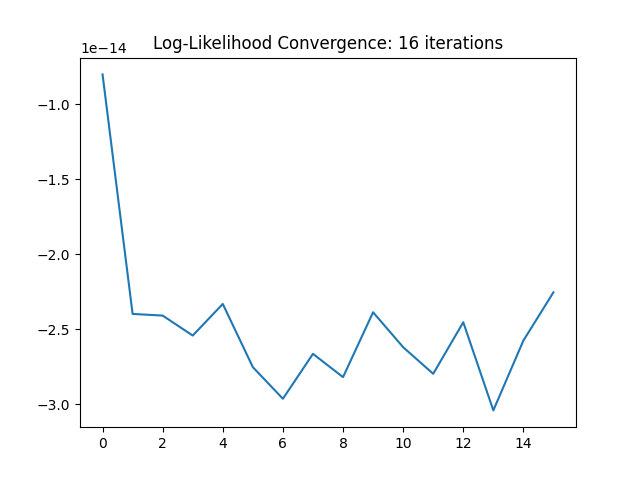
\includegraphics[width=\textwidth, height=.5\textwidth]{images/gmm_LL_conversion.png}
    \end{figure}

\item (20 points) Report the fitted GMM model when EM has terminated in your algorithms as follows:
\begin{itemize}
    \item The numerical weights for each component
    
    My numerical weights are:
    \lstinline{Pi (prior probabilities): [0.5043444 0.4956556]}
    
    \item The mean of each component by mapping it back to the original space and reformatting the vectors into 28-by-28 matrices. These should be displayed as images, ideally corresponding to a kind of "average" of the images.
    My mean values are:
    \lstinline{Mu (mean vectors for each component): [[-5.37469142  0.67257202 -0.92609628  0.77880141],[ 5.46890925 -0.68436215  0.94233066 -0.79245373]]}

    After reversing the PCA and scaling, the output images of each mean vector component are shown below. Clearly, we can see that the GMM means correspond to the 2 and 6 digits. This was not always the case, depending on the random seed.
    \begin{figure}[H]
        \centering
        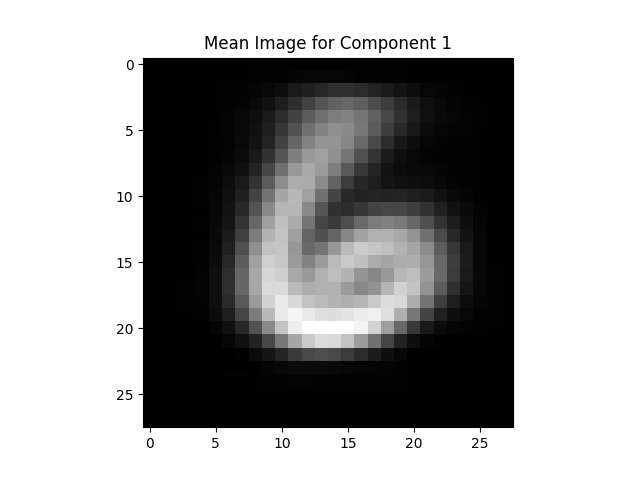
\includegraphics[width=\textwidth, height=.5\textwidth]{images/pc1_mean_gmm.png}
    \end{figure}
    \begin{figure}[H]
        \centering
        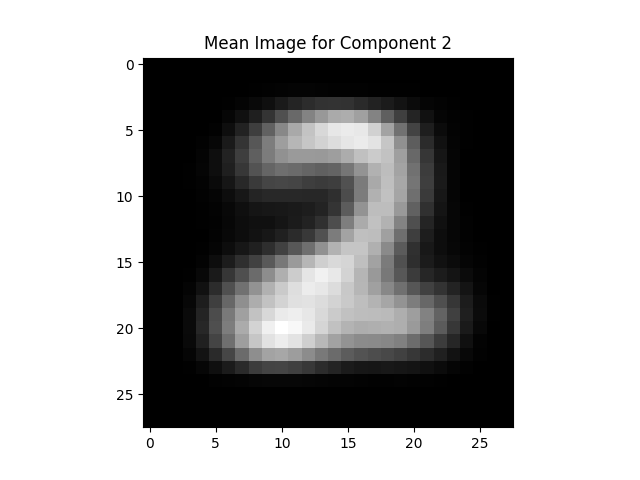
\includegraphics[width=\textwidth, height=.5\textwidth]{images/pc2_mean_gmm.png}
    \end{figure}

    \item Two 4-by-4 covariance matrices by visualizing their intensities (i.e. a gray-scaled image or heatmap.)
    The covariance matrices are shown below:
    \begin{figure}[H]
        \centering
        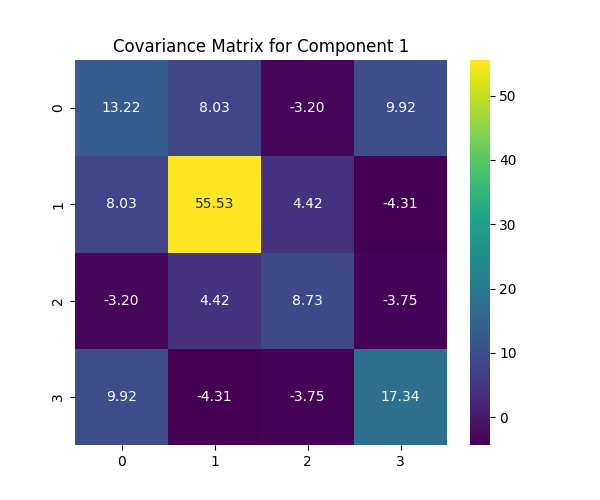
\includegraphics[width=\textwidth, height=.5\textwidth]{images/pc1_cov.png}
    \end{figure}
    \begin{figure}[H]
        \centering
        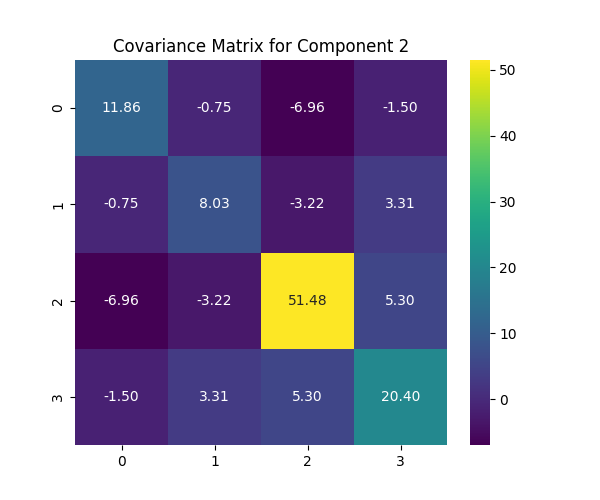
\includegraphics[width=\textwidth, height=.5\textwidth]{images/pc2_cov.png}
    \end{figure}
\end{itemize}

\item (10 points) Use the $\tau_{k}^i$ to infer the labels of the images, and compare with the true labels. Report the mis-classification rate (1 - Accuracy) for digits ``2'' and ``6'' respectively. Perform $K$-means clustering with $K=2$ (you may call a package or use the code from your previous homework). Find out the  mis-classification rate for digits ``2'' and ``6'' respectively, and compare with GMM. Which one achieves the better performance?

To infer the labels of the images, I had to first conver the tau array into labels. For each image, tau contains the responsibility for each of the two Gaussians in our model. In this case, each model should correspond to one of the digits. Therefore, the image label is the tau entry that is greatest. Visually, I could hard-code the corresponding tau component to 2 or 6, but I programmatically determined that using the mode of the labels. In the end, the accuracy metrics of the GMM were very good:

\begin{center}
\begin{tabular}{|c|c|c|c|c|}
\hline
& Gmm 2 & Gmm 6 & Misclassification Rate\\\hline
\textsf{True 2} & 970 & 62 & 0.060\\\hline
\textsf{True 6} & 12 & 946 & 0.013\\\hline
\textsf{Total} & & & 0.037\\\hline
\end{tabular}
\end{center}

After performing K-Means and converting the labels to digits, the accuracy metrics were:
\begin{center}
\begin{tabular}{|c|c|c|c|c|}
\hline
& K-Means 2 & K-Means 6 & Misclassification Rate\\\hline
\textsf{True 2} & 953 & 79 & 0.077\\\hline
\textsf{True 6} & 31 & 927 & 0.032\\\hline
\textsf{Total} & & & 0.055\\\hline
\end{tabular}
\end{center}

In the end, my GMM algorithm outperformed the K-Means algorithm. However, there were many random seed values I tried that did not converge quickly and had worse performance than the K-Means with the same random seeds. Surely, more polished GMM packages handle the initializations better, so I am chalking this up to user error. However, the ease of K-Means for a relatively accurate outcome can be very useful.

\end{enumerate}

\subsection*{4. Correlated features (motivation for PCA) (15 points)}

We will consider a simple question related to our house price prediction with correlated features. You are predicting house prices with two features:
\begin{itemize}
    \item $x_1 =$ number of \textbf{bedrooms}
    \item $x_2 =$ number of \textbf{bathrooms}
\end{itemize}

Suppose the (standardized) features are perfectly correlated: $x_1 = 1.5\,x_2$ for every sample.  
You collect $m=10$ samples and fit a linear model \textbf{with an intercept}:
\[
y = \beta_0 + \beta_1 x_1 + \beta_2 x_2 + \varepsilon .
\]

Let the $n\times 3$ design matrix be $X=[\mathbf{1}^T; \mathbf{x}_1^T; \mathbf{x}_2^T]\in \mathbb R^{3\times m}$. 
Define the \textbf{sample covariance matrix}
\[
G \;=\; \frac{1}{m}\,X X^T.
\]

    \begin{tcolorbox}[colback=gray!10,colframe=gray!60!black,title=Hint]
    Professor Xie covers a similar example in detail in her recorded office hours, and the slides for this are under Module Two: pca\_example.pdf.
    \end{tcolorbox}

\begin{enumerate}
    \item (5 points) Express $G$ analytically in terms of
    \[
    T=\sum_{i=1}^m x_{2,i},\qquad S=\sum_{i=1}^m x_{2,i}^2,
    \]
    using the relation $x_{1,i}=1.5\,x_{2,i}$. Show that $\operatorname{rank}(G)=2$. 

    \begin{align}
    X &= \begin{bmatrix}1 & 1 & 1 & 1 & 1 & 1 & 1 & 1 & 1 & 1\\ 
        1.5x_2^1 & 1.5x_2^2 &1.5x_2^3 &1.5x_2^4 &1.5x_2^5 &1.5x_2^6 &1.5x_2^7&1.5x_2^8&1.5x_2^9&1.5x_2^{10} \\
        x_2^1 & x_2^2 &x_2^3 &x_2^4 &x_2^5 &x_2^6 &x_2^7&x_2^8&x_2^9&x_2^{10} \\
    \end{bmatrix} \\
     G &= \frac{1}{m} X X^T \\
     &= \frac{1}{m}
     \begin{bmatrix}1 & 1 & 1 & 1 & 1 & 1 & 1 & 1 & 1 & 1\\ 
        1.5x_2^1 & 1.5x_2^2 &1.5x_2^3 &1.5x_2^4 &1.5x_2^5 &1.5x_2^6 &1.5x_2^7&1.5x_2^8&1.5x_2^9&1.5x_2^{10} \\
        x_2^1 & x_2^2 &x_2^3 &x_2^4 &x_2^5 &x_2^6 &x_2^7&x_2^8&x_2^9&x_2^{10} \\
    \end{bmatrix} 
     \begin{bmatrix}
        1 & 1.5 x_2^1 & x_2^1 \\
        1 & 1.5 x_2^2 & x_2^2 \\
        1 & 1.5 x_2^3 & x_2^3 \\
        1 & 1.5 x_2^4 & x_2^4 \\
        1 & 1.5 x_2^5 & x_2^5 \\
        1 & 1.5 x_2^6 & x_2^6 \\
        1 & 1.5 x_2^7 & x_2^7 \\
        1 & 1.5 x_2^8 & x_2^8 \\
        1 & 1.5 x_2^9 & x_2^9 \\
        1 & 1.5 x_2^{10} & x_2^{10}
    \end{bmatrix}\\
     &=\frac{1}{m} 
     \begin{bmatrix}
        \sum_{i=1}^m (1\cdot 1) & \sum_{i=1}^m (1\cdot 1.5 x_2^i) & \sum_{i=1}^m (1\cdot x_2^i)\\
        \sum_{i=1}^m (1.5x_2^i \cdot 1) & \sum_{i=1}^m (1.5x_2^i \cdot  1.5x_2^i)& \sum_{i=1}^m (1.5x_2^i \cdot  x_2^i)\\
        \sum_{i=1}^m  (x_2^i \cdot  1)& \sum_{i=1}^m (x_2^i \cdot  1.5x_2^i)& \sum_{i=1}^m (x_2^i \cdot  x_2^i)\\
     \end{bmatrix}\\
     \intertext{Simplify and substitute T and S:}
     &=\frac{1}{m} 
     \begin{bmatrix}
        m & 1.5T & T\\
        1.5T & 2.25S & 1.5S\\
        T & 1.5S& S\\
     \end{bmatrix}\\
     G &=\begin{bmatrix}
        1 & \frac {1.5T} m & \frac T m\\
        \frac {1.5T} m & \frac {2.25S} m & \frac {1.5S} m\\
        \frac T m & \frac {1.5S} m & \frac S m\\
     \end{bmatrix}\\
\end{align}

To begin with, I can see that Row 2 is a scalar multiple of Row 3: $G_2 = 1.5G_3$. This means that one dimension is not independent, so the rank cannot be 3. To prove the rank is 2, I will check the 2x2 minor sub-matrices for non-zero determinants (\cite{se628927}).

\begin{align*}
    \det{
        \begin{bmatrix}
        1 & \frac{1.5T}{m} \\
        \frac{1.5T}{m} & \frac{2.25S}{m}
        \end{bmatrix}
    } &= 1 \cdot \frac{2.25S}{m} - \frac{1.5T}{m} \cdot \frac{1.5T}{m} = \frac{2.25S}{m} - \frac{2.25T^2}{m^2} \ne 0\\
\end{align*}

Therefore, $Rank(G) = 2$.

    
    \item (5 points) Find the the largest eigenvector for $G$, i.e., the weights to combine features, using a mathematical proof.

    Performing eigendecomposition on G:
    \begin{align*}
    G -\lambda I &=\begin{bmatrix}
        1 - \lambda & \frac {1.5T} m & \frac T m\\
        \frac {1.5T} m & \frac {2.25S}{m} - \lambda  & \frac {1.5S} m\\
        \frac T m & \frac {1.5S} m & \frac{S}{m}- \lambda \\
     \end{bmatrix}\\
    det(G -\lambda I) & = \begin{aligned}[t]
        & (1 - \lambda)((\frac {2.25S}{m})(\frac{S}{m}- \lambda)-(\frac {1.5S} m)(\frac {1.5S} m)) \\
        &\quad - (\frac {1.5T} m)((\frac {1.5T} m)(\frac{S}{m}- \lambda)-(\frac {1.5S} m)(\frac T m)) \\ 
        &\quad + (\frac T m)((\frac {1.5T} m)(\frac {1.5S} m)-(\frac {2.25S}{m} - \lambda)(\frac T m))
        \end{aligned}\\
        &= -\lambda^3 + \frac{3.25S}{m}\lambda^2 + \frac{3.25(T^2-S)}{m}\lambda
    \end{align*}

    Characteristic equation is:
    \begin{align*}
    0 &= \lambda(-\lambda^2 + \frac{3.25S}{m}\lambda + \frac{3.25(T^2-S)}{m})
    \end{align*}

    For the zero eigenvalue, the eigenvector is visually calculated since I know it corresponds to the dependent variable: 
    $$u = \begin{bmatrix}
        0 & 1 & -1.5
    \end{bmatrix}$$

    Frankly, the rest of the eigendecomposition is very complex, so I used a SymPy script to perform the rest of the calculation.

    \begin{figure}[H]
        \centering
        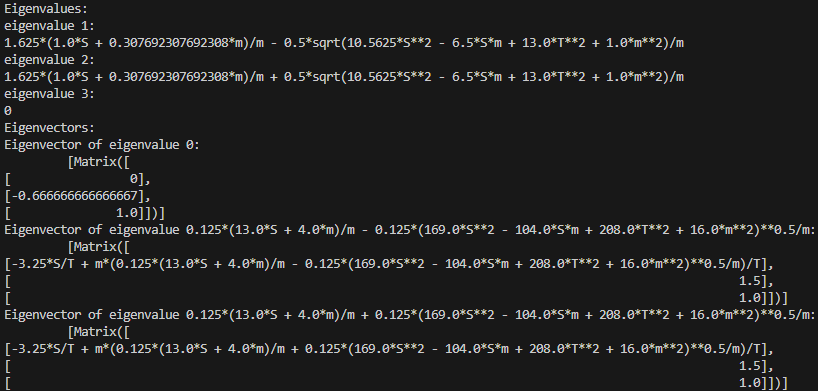
\includegraphics[width=\textwidth, height=.5\textwidth]{images/eigendecomp.png}
    \end{figure}

    What I noticed is that the other eigenvectors have the same second and third values. So the largest eigenvector would be either of those with the largest value in the first spot.

    \item (5 points) (Numerical check) Use the bathroom counts  
    \([1,2,2,3,1,2,3,2,1,2]\) for the 10 homes. Compute $G$ and verify its rank.

    Plugging in the values to get T and S:
    \begin{align*}
    T &= 19\\
    S &= 41\\
    G &= \begin{bmatrix}
        1 & 2.85 & 1.9 \\
        2.85 & 9.225 & 6.15 \\
        1.9 & 6.15 & 4.1
    \end{bmatrix}
    \end{align*}

    As before, dividing rows 1 and 2 by row 3 confirms that row 1 is not a multiple of row 3 and row 2 is $1.5*Row3$. This confirms that the rank is 2.

\end{enumerate}

\pagebreak

\subsection*{5. De-bias review system using EM. [Bonus, 10 points]} 

In this question, we will develop an algorithm to remove individual reviewer's bias from their score. Consider the following problem. There are $P$ papers submitted to a machine learning conference. Each of $R$ reviewers reads each paper, and gives it a score indicating how good he/she thought that paper was. We let $x^{(pr)}$ denote the score that reviewer $r$ gave to paper $p$. A high score means the reviewer liked the paper, and represents a recommendation from that reviewer that it be accepted for the conference. A low score means the reviewer did not like the paper.

We imagine that each paper has some ``intrinsic'' true value that we denote by $\mu_p$, where a large value means it's a good paper. Each reviewer is trying to estimate, based on reading the paper, what $\mu_p$ is; the score reported $x^{(pr)}$ is then reviewer $r$'s guess of $\mu_p$.

However, some reviewers are just generally inclined to think all papers are good and tend to give all papers high scores; other reviewers may be particularly nasty and tend to give low scores to everything. (Similarly, different reviewers may have different amounts of variance in the way they review papers, making some reviewers more consistent/reliable than others.) We let $\nu_r$ denote the ``bias'' of reviewer $r$. A reviewer with bias $\nu_r$ is one whose scores generally tend to be $\nu_r$ higher than they should be.

All sorts of different random factors influence the reviewing process, and hence we will use a model that incorporates several sources of noise. Specifically, we assume that reviewers's scores are generated by a random process given as follows:

\[
y^{(p)} \sim \mathcal{N}(\mu_p, \sigma_p^2)
\]
\[
z^{(r)} \sim \mathcal{N}(\nu_r, \tau_r^2)
\]
\[
x^{(pr)}|y^{(p)}, z^{(r)} \sim\mathcal{N}(y^{(p)}+ z^{(r)}, \sigma^2).
\]
The variables $y^{(p)}$ and $z^{(r)}$ are independent; the variables $(x,y,z)$ for different paper-reviewer pairs are also jointly independent. Also, we only ever observe the $x^{(pr)}$s; thus, the $y^{(p)}$s and $z^{(r)}$s are all latent random variables.
 
We would like to estimate the parameters $\mu_p$, $\sigma_p^2$, $\nu_r$, $\tau_r^2$. If we obtain good estimates of the papers ``intrinsic values'' $\mu_p$, these can then be used to make acceptance/rejection decisions for the conference. 

We will estimate the parameters by maximizing the marginal likelihood of the data $\{x^{(pr)}; p = 1,\ldots,P,r = 1,\ldots,R\}$. This problem has latent variables $y^{(p)}$s and $z^{(r)}$s, and the maximum likelihood problem cannot be solved in closed form. So, we will use EM. 

{\bf Your task} is to derive the EM update equations. For simplicity, you need to treat only $\{\mu_p,\sigma_p^2; p = 1\ldots,P\}$ and $\{\nu_r,\tau_r^2;r = 1...R\}$ as parameters, i.e. treat $\sigma^2$ (the conditional variance of $x^{(pr)}$ given $y^{(p)}$ and $z^{(r)}$) as a fixed, known constant.

\begin{enumerate}[label*=\arabic*.]
\item Derive the E-step (5 points)

\begin{enumerate}[label*=\arabic*.]
\item  The joint distribution $p(y^{(p)},z^{(r)},x^{(pr)})$ has the form of a multivariate Gaussian density. Find its associated mean vector and covariance matrix in terms of the parameters $\mu_p$, $\sigma_p^2$, $\nu_r$, $\tau_r^2$ and $\sigma^2$.
[Hint: Recognize that $x^{(pr)}$ can be written as $x^{(pr)} = y^{(p)} + z^{(r)} + \epsilon^{(pr)}$, where $\epsilon^{(pr)} \sim \mathcal{N}(0, \sigma^2)$ is independent Gaussian noise.

\item Derive an expression for $Q_{pr}(\theta'|\theta)  = \mathbb{E}[\log p(y^{(p)}, z^{(r)}, x^{(pr)})|x^{(pr)},\theta]$ using the conditional distribution $p(y^{(p)},z^{(r)}|x^{(pr)})$ (E-step) (Hint, you may use the rules for conditioning on subsets of jointly Gaussian random variables.) % (see the notes
\end{enumerate}

\item (5 points) Derive the M-step to update the parameters $\mu_p$, $\sigma_p^2$, $\nu_r$, and $\tau_r^2$. [Hint: It may help to express an approximation to the likelihood in terms of an expectation with respect to $(y^{(p)}, z^{(r)})$ drawn from a distribution with density $Q_{pr}(y^{(p)}, z^{(r)})$.]

\end{enumerate}

{\bf Remark:} John Platt (whose SMO algorithm you've seen) implemented a method quite similar to this one to estimate the papers' true scores. (There, the problem was a bit more complicated because not all reviewers reviewed every paper, but the essential ideas are the same.) Because the model tried to estimate and correct for reviewers' biases, its estimates of the paper's value were significantly more useful for making accept/reject decisions than the reviewers' raw scores for a paper.




\printbibliography



\end{document}
